\section{Применение уравнений электростатики}

	Мы записали два уравнения:
	\begin{eqnarray}
		& \oint E_n \d{S}=\dfrac{q_{\Sigma}}{\varepsilon_0}, \\
		& \oint E_l \d{l}=0.
	\end{eqnarray}
	Сформулируем \i{принцип симметрии}\index{Принцип!симметрии}: если некоторая система зарядов переходит сама в себя при некотором преобразовании симметрии (поворот, сдвиг, отражение), то картина создаваемого поля переходит сам а в себя при этом преобразовании. \par

	Рассмотрим равномерно заряженную сферу \index{Сфера!заряженная} радиуса $R$. При повороте вокруг прямой $r$ вектор $\vec{E}$ переходит сам в себя. В каждой точке сферы радиуса $r$ поле \index{Поле} нормально и равно $E$, а 
	\begin{equation}
		\oint E_n \d{S}=E\cdot 4\pi r^2=\frac{q(r)}{\varepsilon_0},
	\end{equation}
	где $q(r)$ -- заряд внутри сферы радиуса $r$ с центром в той же точке. Отсюда
	\begin{equation}
		E=\frac{1}{4\pi r^2}\frac{q(r)}{\varepsilon_0}.
	\end{equation}
	Если $r<R$, то поле $E$ равно нулю, так как $q(r)=0$. При $r\qe R$ $q(r)=q$. Окончательно
	\begin{equation}
		E(r)=	\begin{cases}
					0,& \text{$0\le r<R$},\\
					k\dfrac{q}{r^2},& \text{$r\qe R$}.
				\end{cases}
	\end{equation}
	Для поля однородно заряженного шара запишем снова: $E(r)=k\dfrac{q(r)}{r^2}$. В силу распределения заряда запишем
		$$\dfrac{q(r)}{q}=\frac{V(r)}{V}=\frac{r^3}{R^3},$$
	откуда
		$$q(r)=q\frac{r^3}{R^3},$$
	а
	\begin{equation}
		E(r)=	\begin{cases}
					kq\dfrac{r}{R^3},& \text{$0\le r<R$},\\
					k\dfrac{q}{r^2},& \text{$r\qe R$}.
				\end{cases}
	\end{equation}
	\begin{figure}[t]
		\centering
		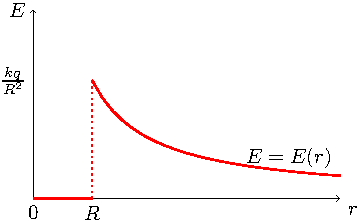
\includegraphics[scale=2]{./img/plot1/plot1.pdf}
		\caption{График поля в зависимости от расстояния $E=E(r)$ для однородно заряженной сферы}
	\end{figure}
	\begin{figure}[t]
		\centering
		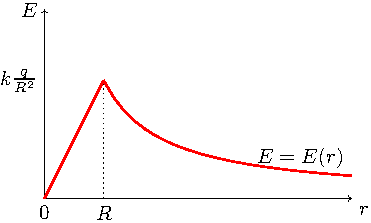
\includegraphics[scale=2]{./img/plot2/plot2.pdf}
		\caption{График поля в зависимости от расстояния $E=E(r)$ для однородно заряженного шара}
	\end{figure}
	Найдем зависимость потенциала от расстояния $\varphi=\varphi(r)$ для обоих случаев. Перепишем~(\ref{phiderivative}) как $\d{\varphi}=-E\d{r}$, откуда
	\begin{equation}
		\varphi(r)=-\int E\d{r}.
	\end{equation}
	Проинтегрируем функцию $E=E(r)$ для сферы, получим
	\begin{equation}
		\varphi(r)=\begin{cases}
						C_1,& \text{$0\le r<R$},\\
						k\dfrac{q}{r} + C_2,& \text{$r\qe R$}.
					\end{cases}
	\end{equation}
	Выясним характер констант интегрирования $C_1$ и $C_2$. Положим $C_2$ равной нулю и сформулируем принцип\index{Принцип!непрерывности потенциала}: если в любой точке простарнства поле конечно, то потенциал непрерывен в этой точке. В самом деле, если потенциал в этой точке непрерывен, то за конечное время поле может совершить бесконечную работу при переносе заряда\index{Заряд} через эту точку, что обязательно чему-то там противоречит. Тогда,
		$$\varphi(R)=\lim_{r\rightarrow R^-} \varphi(r)=C_1.$$
	Окончательно
	\begin{equation}
		\varphi(r)=\begin{cases}
						k\dfrac{q}{R},& \text{$0\le r<R$},\\
						k\dfrac{q}{r},& \text{$r\qe R$}.
					\end{cases}
	\end{equation}
	\begin{figure}[t]
		\centering
		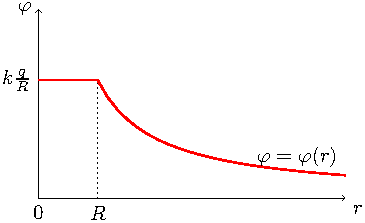
\includegraphics[scale=2]{./img/plot3/plot3.pdf}
		\caption{График потенциала в зависимости от расстояния $\varphi=\varphi(r)$ для однородно заряженной сферы}
	\end{figure}
	Проделаем то же для шара:
	\begin{equation}
		\varphi(r)=\begin{cases}
						-kq\dfrac{r^2}{2R^3}+C_1,& \text{$0\le r<R$},\\
						k\dfrac{q}{r} + C_2,& \text{$r\qe R$}.
					\end{cases}
	\end{equation}
	$C_2=0$. В силу непрерывности
		$$\varphi(R)=k\frac{q}{R}=C_1-kq\frac{R^2}{2R^3}, \quad C_1=\frac{3}{2}k\frac{q}{R}.$$
	Окончательно
	\begin{equation}
		\varphi(r)=\begin{cases}
						-\dfrac{1}{2}kq\dfrac{r^2}{R^3}+\dfrac{3}{2}k\dfrac{q}{R},& \text{$0\le r<R$},\\
						k\dfrac{q}{r},& \text{$r\qe R$}.
					\end{cases}
	\end{equation}
	Заметим, что график этой функции гладок в точке $R$ в силу её дифференцируемости в этой точке. 
	\begin{figure}[t]
		\centering
		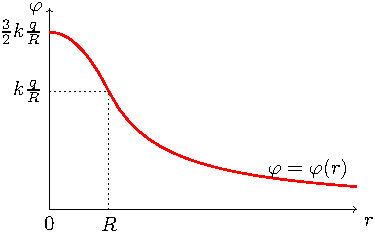
\includegraphics[scale=2]{./img/plot4/plot4.pdf}
		\caption{График потенциала в зависимости от расстояния $\varphi=\varphi(r)$ для однородно заряженного шара}
	\end{figure}